\section{Beispiel 3}

F"ur einen PNP-Transistor und einen p-Kanal MOSFET sollten bei unterschiedlichen Temperaturen die "Ubertragungs- und Ausgangskennlinienscharen simuliert werden. Abbildungen \ref{fig:3_pnp_transfer} und \ref{fig:3_pnp_output} zeigen die "Ubertragungs- und Ausgangskennlinie f"ur einen PNP-Transistor vom Typ Q2N3906, Abbildungen \ref{fig:3_pmos_transfer} und \ref{fig:3_pmos_output} zeigen die "Ubertragungs- und Ausgangskennlinie f"ur einen p-Kanal MOSFET vom Typ IRF9140. Dabei wurden die Simulationen f"ur mehrere $V_{CE}$ bzw. $V_{DS}$ mit Hilfe eines \emph{Nested Sweep} durchgef"uhrt (es wurden nicht zu viele Werte gew"ahlt, sodass das Diagramm "ubersichtlich bleibt). Weiters wurden die Simulationen bei unterschiedlichen Temperaturen durchgef"uhrt. Die Kurven sind beschriftet und haben in allen Diagrammen die gleiche Farbgebung (gr"un...-10°C, rot...27°C, blau...85°C). Man kann die Temperaturabh"angigkeit von $V_{BE}$ des PNP-Transistors gut erkennen.

\begin{figure}%[h!]
	\centering
	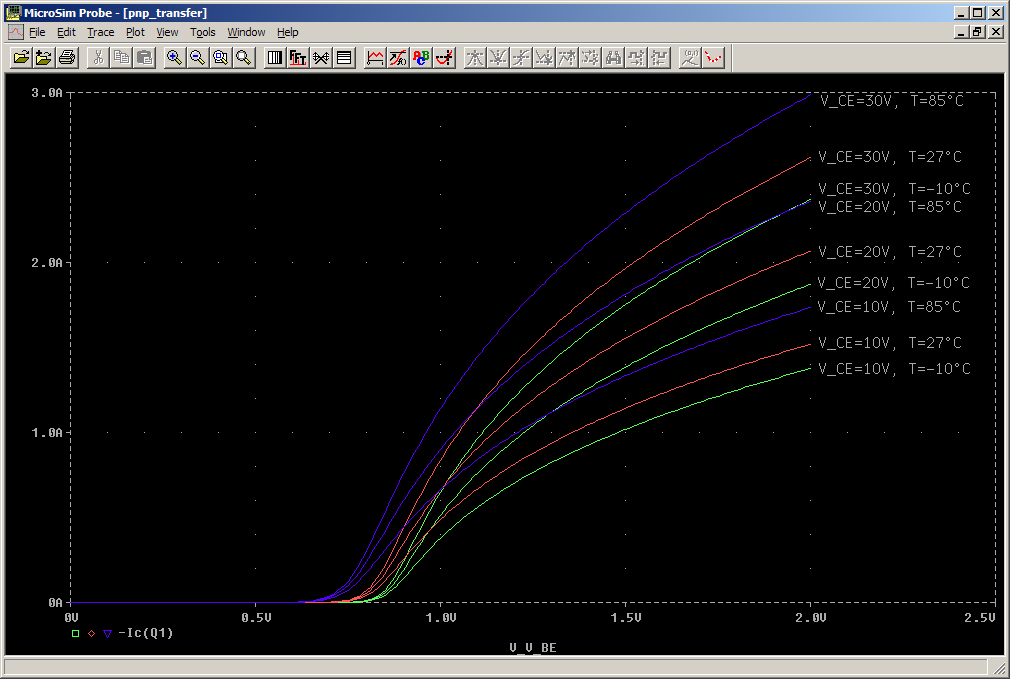
\includegraphics[width=\textwidth]{fig/ue2_ex3_pnp_transfer.PNG}
	\caption{"Ubertragungskennlinie des Q2N3906}
	\label{fig:3_pnp_transfer}
\end{figure}

\begin{figure}%[h!]
	\centering
	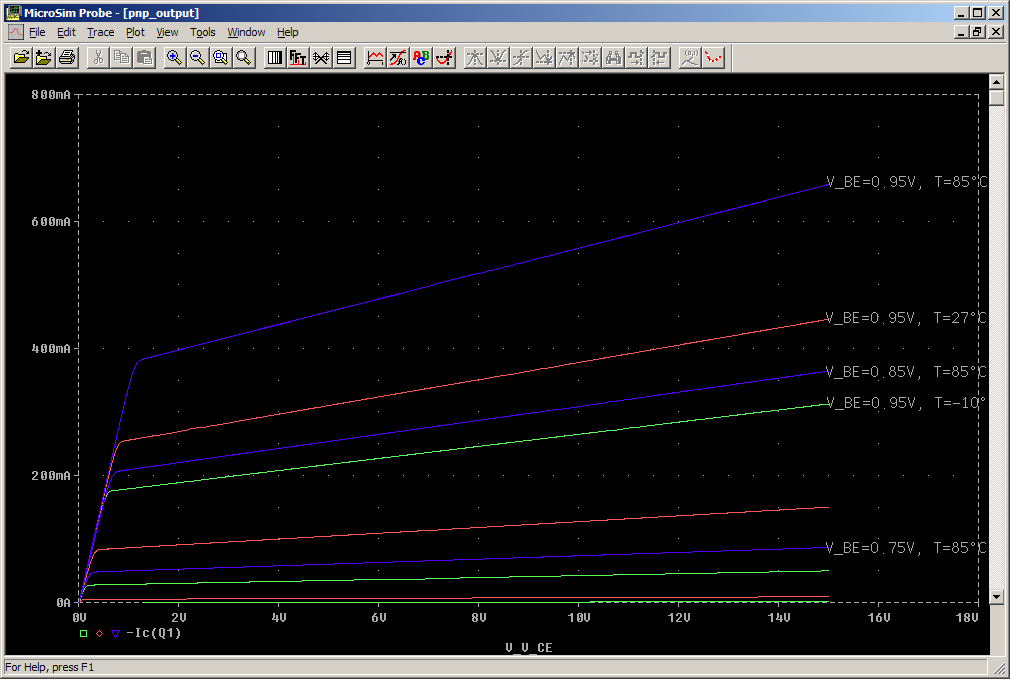
\includegraphics[width=\textwidth]{fig/ue2_ex3_pnp_output.PNG}
	\caption{Ausgangskennlinie des Q2N3906}
	\label{fig:3_pnp_output}
\end{figure}

\begin{figure}%[h!]
	\centering
	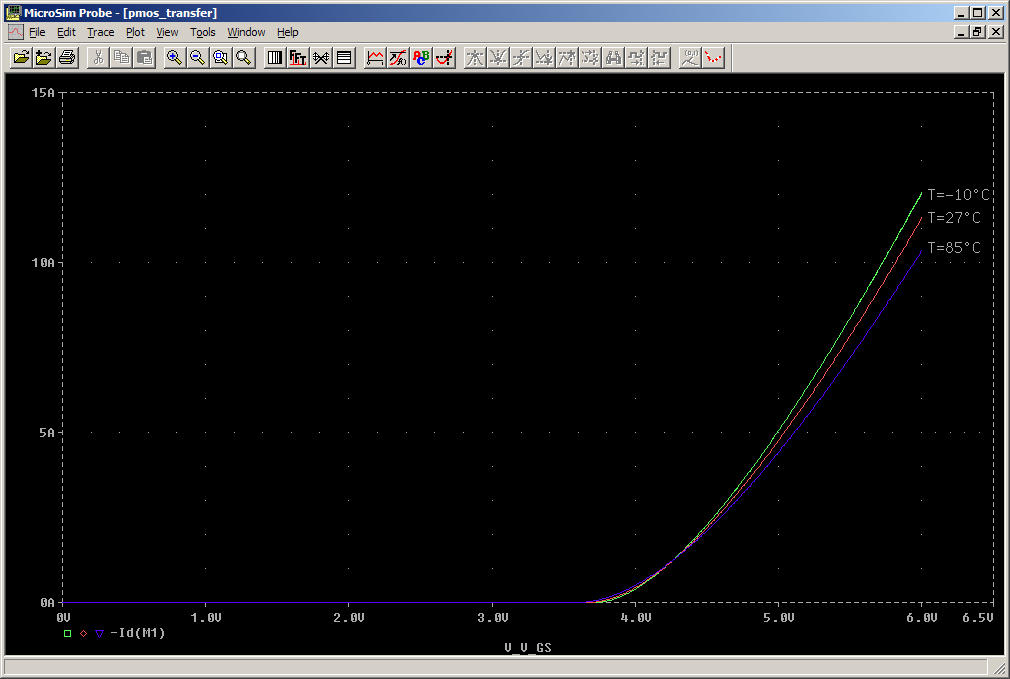
\includegraphics[width=\textwidth]{fig/ue2_ex3_pmos_transfer.PNG}
	\caption{"Ubertragungskennlinie des IRF9140}
	\label{fig:3_pmos_transfer}
\end{figure}

\begin{figure}%[h!]
	\centering
	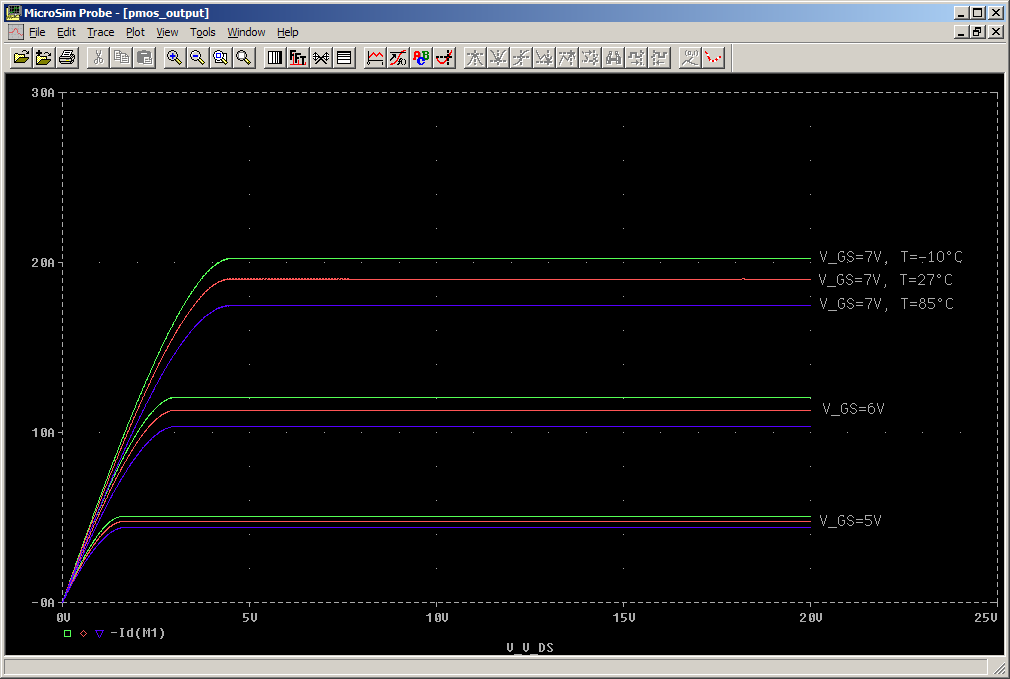
\includegraphics[width=\textwidth]{fig/ue2_ex3_pmos_output.PNG}
	\caption{Ausgangskennlinie des IRF9140}
	\label{fig:3_pmos_output}
\end{figure}


Abbildungen \ref{fig:3_pnp_s} und \ref{fig:3_pnp_s_norm} zeigen die Steilheit des PNP-Transistors $S = \frac{dI_C}{dV_{BE}}$ und die auf den Strom normierte Steilheit $S_{norm} = \frac{S}{I_C}$. Die maximalen Steilheiten werden im Bereich von $V_{BE}$ erreicht, bei dem der Transistor zu leiten beginnt.

\begin{figure}%[h!]
	\centering
	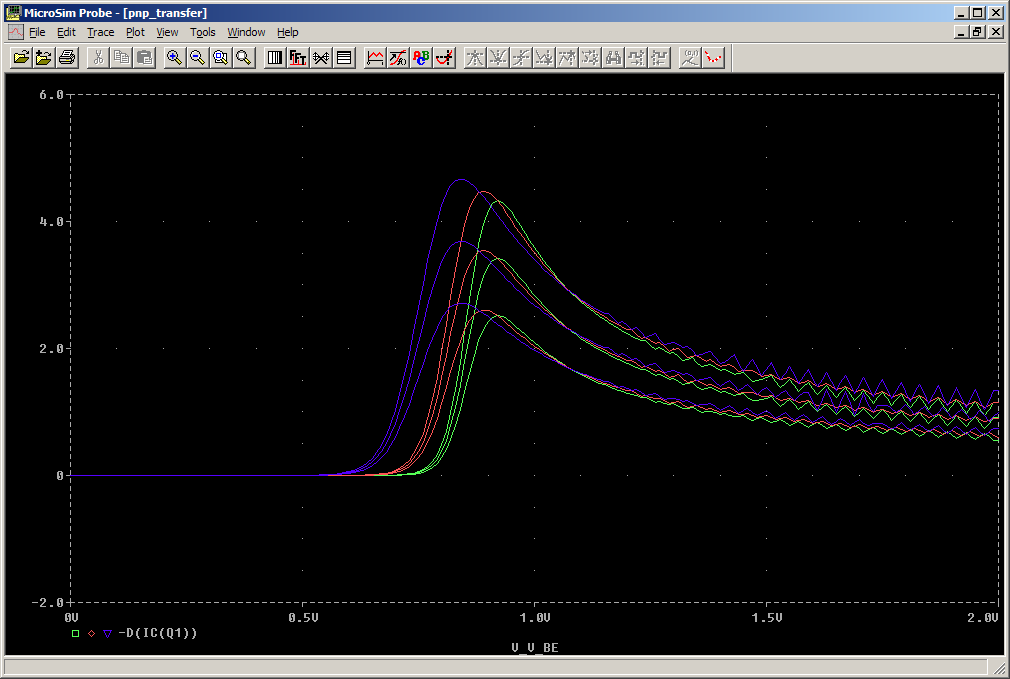
\includegraphics[width=\textwidth]{fig/ue2_ex3_pnp_s.PNG}
	\caption{Steilheit des Q2N3906}
	\label{fig:3_pnp_s}
\end{figure}

\begin{figure}%[h!]
	\centering
	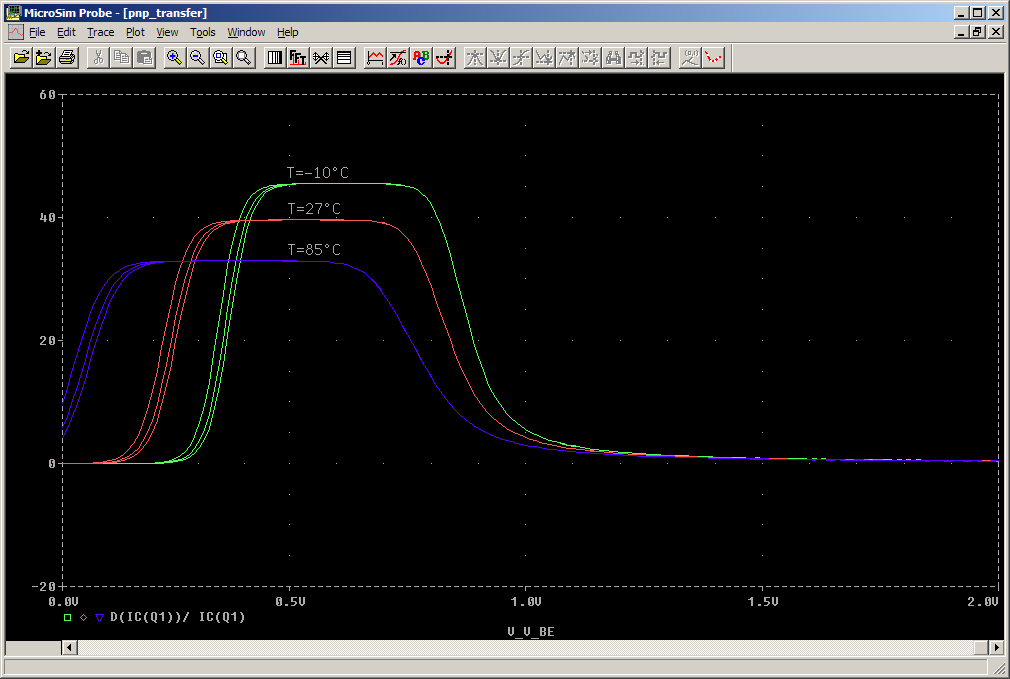
\includegraphics[width=\textwidth]{fig/ue2_ex3_pnp_s_norm.PNG}
	\caption{Normierte Steilheit des Q2N3906}
	\label{fig:3_pnp_s_norm}
\end{figure}

Abbildungen \ref{fig:3_pmos_s} und \ref{fig:3_pmos_s_norm} zeigen die Steilheit des p-Kanal MOSFET $g_m = \frac{dI_D}{dV_{GS}}$ und die auf den Strom normierte Steilheit $g_{m_{norm}} = \frac{g_m}{I_D}$. Man erkennt, dass die maximale (normierte) Steilheit nur in einem sehr schmalen Bereich verf"ugbar ist.

\begin{figure}%[h!]
	\centering
	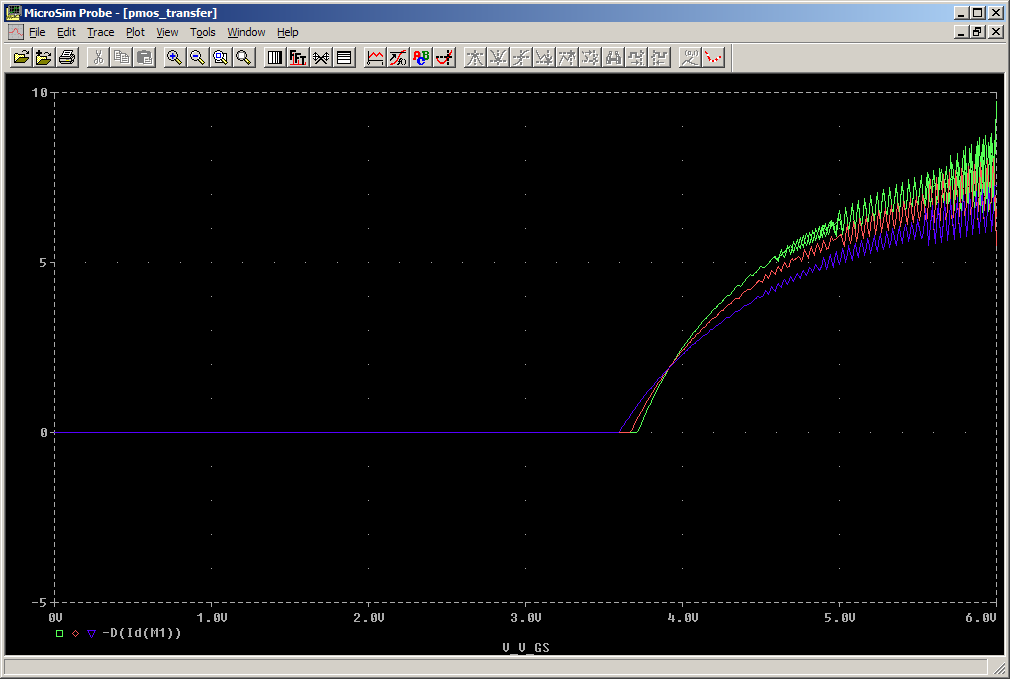
\includegraphics[width=\textwidth]{fig/ue2_ex3_pmos_s.PNG}
	\caption{Steilheit des IRF9140}
	\label{fig:3_pmos_s}
\end{figure}

\begin{figure}%[h!]
	\centering
	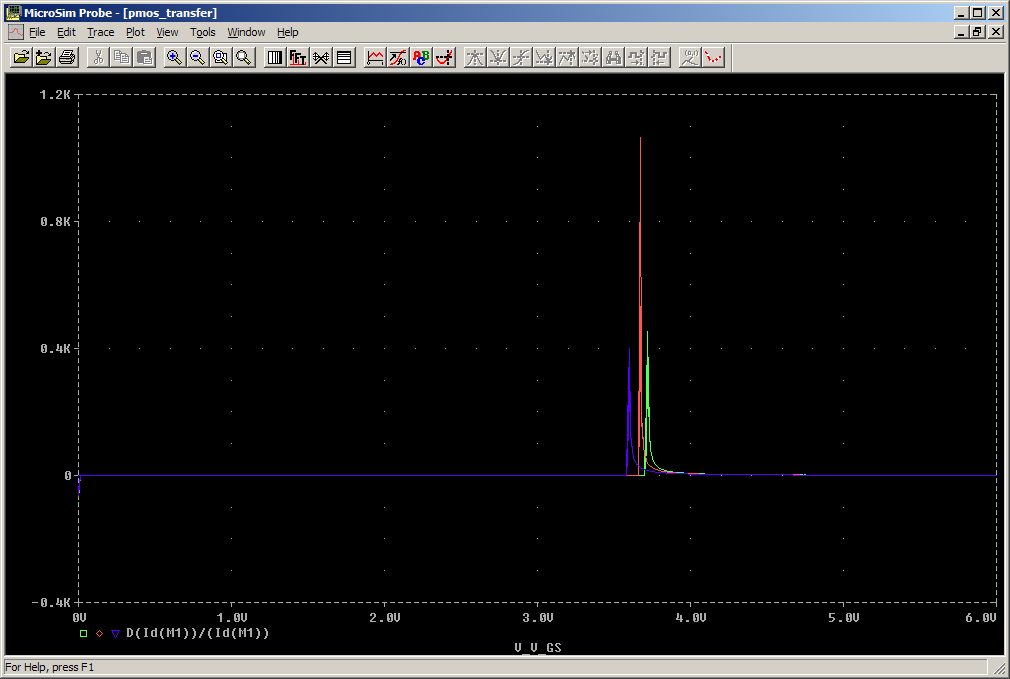
\includegraphics[width=\textwidth]{fig/ue2_ex3_pmos_s_norm.PNG}
	\caption{Normierte Steilheit des IRF9140}
	\label{fig:3_pmos_s_norm}
\end{figure}

